\documentclass[a4paper, 14pt]{extarticle}

% Поля
%--------------------------------------
\usepackage{geometry}
\geometry{a4paper,tmargin=2cm,bmargin=2cm,lmargin=3cm,rmargin=1cm}
%--------------------------------------


%Russian-specific packages
%--------------------------------------
\usepackage[T2A]{fontenc}
\usepackage[utf8]{inputenc}
\usepackage[english, main=russian]{babel}
\usepackage{cmap}
%--------------------------------------

\usepackage{textcomp}
\usepackage{amssymb}

% Красная строка
%--------------------------------------
\usepackage{indentfirst}               
%--------------------------------------             


%Graphics
%--------------------------------------
\usepackage{graphicx}
\graphicspath{ {./images/} }
\usepackage{wrapfig}
%--------------------------------------

% Полуторный интервал
%--------------------------------------
\linespread{1.3}                    
%--------------------------------------

%Выравнивание и переносы
%--------------------------------------
% Избавляемся от переполнений
\sloppy
% Запрещаем разрыв страницы после первой строки абзаца
\clubpenalty=10000
% Запрещаем разрыв страницы после последней строки абзаца
\widowpenalty=10000
%--------------------------------------

%Списки
\usepackage{enumitem}

%Подписи
\usepackage{caption} 

%Гиперссылки
\usepackage{hyperref}

\hypersetup {
	unicode=true
}

%Рисунки
%--------------------------------------
\DeclareCaptionLabelSeparator*{emdash}{~--- }
\captionsetup[figure]{labelsep=emdash,font=onehalfspacing,position=bottom}
%--------------------------------------

\usepackage{tempora}
\usepackage{amsmath}
\usepackage[dvipsnames]{xcolor}
\usepackage{listings}
\lstset{
  belowcaptionskip=1\baselineskip,
  breaklines=true,
  frame=L,
  xleftmargin=\parindent,
  language=Java,
  showstringspaces=false,
  basicstyle=\footnotesize\ttfamily,
  keywordstyle=\bfseries\color{blue},
  commentstyle=\itshape\color{purple},
  identifierstyle=\color{black},
  stringstyle=\color{red},
  numbers=left,           
  numberstyle=\tiny\color{gray}, 
  numbersep=10pt,      
  % ------------------------------
}

%--------------------------------------
%			НАЧАЛО ДОКУМЕНТА
%--------------------------------------

\begin{document}

%--------------------------------------
%			ТИТУЛЬНЫЙ ЛИСТ
%--------------------------------------
\begin{titlepage}
\thispagestyle{empty}
\newpage


%Шапка титульного листа
%--------------------------------------
\vspace*{-60pt}
\hspace{-65pt}
\begin{minipage}{0.3\textwidth}
\hspace*{-20pt}\centering

\includegraphics[width=\textwidth]{emblem}
\end{minipage}
\begin{minipage}{0.67\textwidth}\small \textbf{
\vspace*{-0.7ex}
\hspace*{-6pt}\centerline{Министерство науки и высшего образования Российской Федерации}
\vspace*{-0.7ex}
\centerline{Федеральное государственное бюджетное образовательное учреждение }
\vspace*{-0.7ex}
\centerline{высшего образования}
\vspace*{-0.7ex}
\centerline{<<Московский государственный технический университет}
\vspace*{-0.7ex}
\centerline{имени Н.Э. Баумана}
\vspace*{-0.7ex}
\centerline{(национальный исследовательский университет)>>}
\vspace*{-0.7ex}
\centerline{(МГТУ им. Н.Э. Баумана)}}
\end{minipage}
%--------------------------------------

%Полосы
%--------------------------------------
\vspace{-25pt}
\hspace{-35pt}\rule{\textwidth}{2.3pt}

\vspace*{-20.3pt}
\hspace{-35pt}\rule{\textwidth}{0.4pt}
%--------------------------------------

\vspace{1.5ex}
\hspace{-35pt} \noindent \small ФАКУЛЬТЕТ\hspace{80pt} <<Информатика и системы управления>>

\vspace*{-16pt}
\hspace{47pt}\rule{0.83\textwidth}{0.4pt}

\vspace{0.5ex}
\hspace{-35pt} \noindent \small КАФЕДРА\hspace{50pt} <<Теоретическая информатика и компьютерные технологии>>

\vspace*{-16pt}
\hspace{30pt}\rule{0.866\textwidth}{0.4pt}
  
\vspace{11em}

\begin{center}
\Large {\bf Лабораторная работа № 10} \\ 
\large {\bf по курсу <<Языки и методы программирования>>} \\ 
\large <<Реализация итераторов на языке C++>>
\end{center}\normalsize

\vspace{8em}


\begin{flushright}
  {Студент группы ИУ9-21Б Воронков А. С.\hspace*{15pt} \\
  \vspace{2ex}
  Преподаватель Посевин Д. П.\hspace*{15pt}}
\end{flushright}

\bigskip

\vfill
 

\begin{center}
\textsl{Москва 2026}
\end{center}
\end{titlepage}
%--------------------------------------
%		КОНЕЦ ТИТУЛЬНОГО ЛИСТА
%--------------------------------------

\renewcommand{\ttdefault}{pcr}

\setlength{\tabcolsep}{3pt}
\newpage
\setcounter{page}{2}

\section{Цель}\label{Sect::task}
\par 
Данная работа предназначена для приобретения навыков разработки контейнерных классов с итераторам. 

\pagebreak
\section{Практическая реализация}
\par
Код файла iter.cpp
\begin{lstlisting}
#include <iostream>
#include <vector>

using namespace std;

class Integers
{
    public:
        class Iterator
        {
            public:
                using iterator_category = std::forward_iterator_tag;
                using difference_type   = std::ptrdiff_t;
                using value_type        = int;
                using pointer           = int*;
                using reference         = int&;

                Iterator(pointer ptr, pointer end) : ptr(ptr), end(end) 
                {
                    while (this->ptr != end && *this->ptr >= 0)
                    {
                        ++this->ptr;
                    }
                }

                reference operator*() const {return *ptr;}
                pointer operator->() const {return ptr;}

                Iterator& operator++() 
                {
                    ++ptr;
                    while (ptr != end && *ptr >= 0)
                    {
                        ++ptr;
                    } 
                    return *this; 
                }
                Iterator operator++(int) { Iterator tmp = *this; ++(*this); return tmp; }
                friend bool operator== (const Iterator& a, const Iterator& b) { return a.ptr == b.ptr; };
                friend bool operator!= (const Iterator& a, const Iterator& b) { return a.ptr != b.ptr; }; 

            private:
                pointer ptr;
                pointer end;
        };

        vector<int> data;
        Integers() {}
        Integers(initializer_list<int> x)
        {
            data = x;
        }
        void Add(int x)
        {
            data.push_back(x);
        }
        Iterator begin() {return Iterator(data.data(), data.data() + data.size());}
        Iterator end() {return Iterator(data.data() + data.size(), data.data() + data.size());}
};

int main()
{
    Integers in2 = Integers({124, -1, 243, -5, -6, 3, -9});
    for (int i = 0; i < in2.data.size(); i++){
        cout << in2.data[i] << endl;
    }
    cout << "negative" << endl;
    for (int x : in2) {
        cout << x << " ";
    }
    cout << endl;
    return 1;
}
\end{lstlisting}


\begin{center}
    \nopagebreak
    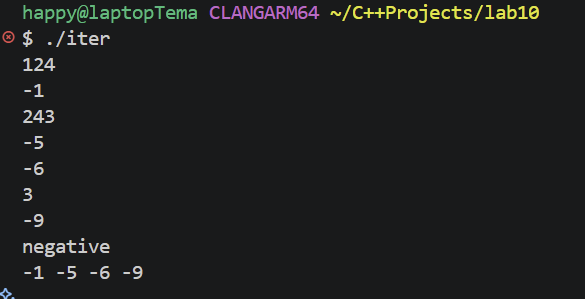
\includegraphics[width=0.85\textwidth]{lab10_1}
    \captionsetup{justification=centering}
    \captionof{figure}{Результат работы программы}
\end{center}

\section{Вывод}
В данной лабораторной работе был получен навык написания итераторов
\end{document}